\documentclass[11pt]{scrartcl}
\usepackage{amsmath}
\usepackage{amssymb}
\usepackage[ngerman]{babel}
\usepackage[pdftex]{graphicx}
\usepackage{epstopdf}
\usepackage{hyperref}
\usepackage[utf8]{inputenc}
\usepackage{verbatim}

\graphicspath{{./}{plots/}}

\title{VDVC Survey}
\author{Patrik Schönfeldt}
\date{\today}

\begin{document}
\maketitle

\section{Beschreibung der Stichprobe}
Der erste Teil der VDVC-Umfrage (künftig: \emph{2013}) wurde über insgesamt 14 Tage
vom 23. Dezember 2013 bis zum 6. Januar 2014 durchgeführt.
1417 Personen haben diesen Teil abgeschlossen.
Der zweite und dritte Teil (künftig: \emph{2014} und \emph{2015})
wurde im Dezember 2014 bzw. 2015 durchgefüht,
die Zahl der komplett abgeschlossenen Fragebögen für diese Jahre beträgt 
1942 (2014) respektive 1356 (2015).
In jedem Jahr wurde bei den Communities \emph{For Uncut!},
\emph{Stigma-Videospiele/VDVC} und \emph{World of Players} für die Umfrage
geworben.
2014 ließ sich ein signifikanter Anteil der Teilnehmer auf einen
Hinweis bei \emph{GameStar} und \emph{GamePro} zurückführen,
2015 gab es einen Hinweis vonseiten \emph{Electronic Arts}.

Da in jedem Jahr neu für die Umfrage geworben wurde und auch keine
Identifikaton der selben Teilnehmer über mehrere Jahre erfolgt,
ist eine statistische Betrachtung der Stichproben der Erhebungsjahre
geboten,
um Vergleichbarkeit zwischen den Jahren herzustellen und deren
statistische Abhängigkeit anschätzen zu können.
Außerdem kann die folgende Untersuchung
Aufschluss über die Repräsentativität der Umfrage geben.


\subsection{Altersstruktur}

\begin{figure}[htbp]
	\centering
	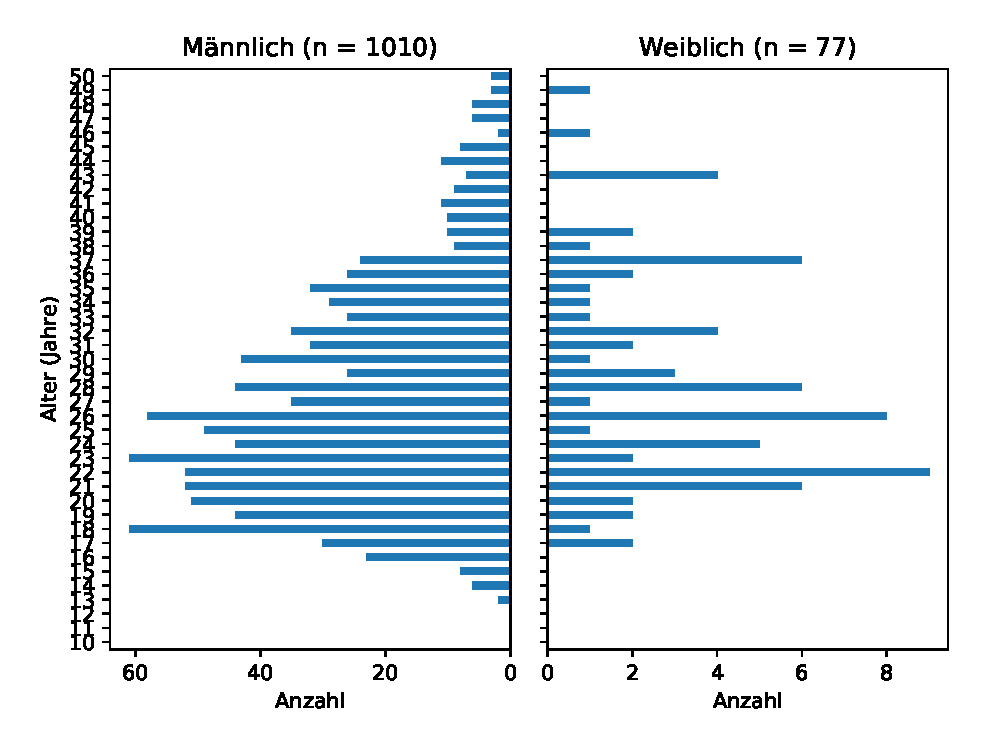
\includegraphics[width=15cm]{vgl/alter}
	\caption[Altersstruktur]
	{Altersstruktur des Teilnahmefelds.}
	\label{fig:alter}
\end{figure}

Die Altersstruktur (Abb.~\ref{fig:alter}) folgt über
den kompletten Erhebungszeitraum einem	ähnlichen Muster:
Jeweils gibt es kaum Teilnehmer unter 15 Jahren,
ab 18 Jahren erreicht die Verteilung ein Plateau.
Zwischen 40 und 50 Jahren sind nur wenige, noch älter kaum noch Teilnehmer.
Es ist im Laufe der Untersuchung eine leichte Verschiebung hin zu höherem
Alter zu beobachten, die jedoch weniger als ein Jahr pro Jahrgang der Umfrage
beträgt.



\subsection{Geschlechter}

\begin{figure}[htbp]
	\centering
	\includegraphics[width=0.33\linewidth]{2013/geschlecht-rel}\hfill
	\includegraphics[width=0.33\linewidth]{2014/geschlecht-rel}\hfill
	\includegraphics[width=0.33\linewidth]{2015/geschlecht-rel}
	\caption{Geschlechter}
	\label{fig:geschlecht}
\end{figure}

\subsection{Zusammenfassung}

Der teilnehmende Personenkreis ist über die Jahre nicht konstant geblieben.
Für diese Aussage sprechen schon die der Hinweise an verschiedenen Stellen,
eindeutig belegt wird sie durch die Entwicklung der Altersstruktur,
die sich pro Jahr der Erhebung weniger als ein Jahr zu höherem Alterbewegt.

Es ist davon auszugehen, dass es eine große Zahl von Personen gibt,
die in mehreren Jahren einen Fragebogen ausgefüllt haben.
Aus diesem Grund können die Stichproben mehrerer Jahre
nicht als unabhängig angesehen werden.
Für die geplante Untersuchung von mehrjährigen Trends
ist die statistische Un-/ Abhängigkeit der Stichproben jedoch nicht von Relevanz,
solange Vergleichbarkeit besteht.

\clearpage
\bibliography{VDVC-Survey}{}
\bibliographystyle{alpha}

\end{document}
